Til lokalisering af robotten anvendes en \kinect (se evt. \cref{kinect:argumentation}).
Denne er udstyret med et farvekamera (se evt. \cref{kinect:farvekamera}), der vil blive anvendt til at bestemme robottens placering.
Ved at udstyre robotten med to mærkninger i klare farver, vil det på billeder fra Kinecten være muligt at lokalisere robotten.

I det følgende beskrives den anvendte metode til lokalisering af robotten.
Først beskrives den overordnede metode, hvorefter forbedringer af metoden præsenteres.

\section{Farveforskel}\label{tracking:colordiff}
%Beskrivelse af den metode der anvendes til at beskrive forskellen mellem farver
Lokalisering af robotten foretages som udgangspunkt ud fra \'et billede.
Det vil sige, at systemet skal være i stand til at lokalisere robotten ud fra \'et billede alene.
Som beskrevet ovenfor udstyres robotten med to mærkninger i klare farver, som skal spores.
Det er altså målet at finde de dele af et enkelt billede, der matcher bestemte farver.

\subsection{Match af farver}
For at vurdere om to farver matcher hinanden, må det først gøres klart, at det ikke kan forventes at matche en farve eksakt.
Til dette spiller faktorer som lys og skygge for stor en rolle.
I stedet tages der udgangspunkt i en søgt farve, og ud fra denne ledes der efter alle \textit{nære} farver.
Til dette formål betragtes den farve-repræsentation der arbejdes med.
Farver repræsenteres ved tre værdier; rød, grøn og blå (også kaldet RGB), der angiver alle de mulige farver for en pixel i et billede.
Ved at betragte de tre farver som hver sin dimension i et tredimensionelt rum, kan farver repræsenteres som vektorer.
Hermed bliver det muligt at tale om forskellen på to farver som \textit{afstanden mellem to farver}.

\begin{figure}
\centering
\tdplotsetmaincoords{60}{110}
\begin{tikzpicture}[scale=5,tdplot_main_coords]

%set up some coordinates 
%-----------------------
\coordinate (O) at (0,0,0);
\tdplotsetcoord{P1}{1.1}{60}{30}
\tdplotsetcoord{P2}{1.5}{40}{60}

%draw figure contents
%--------------------

%draw the main coordinate system axes
\draw[ultra thick,red,->] (0,0,0) -- (1,0,0) node[anchor=north east]{$r$};
\draw[ultra thick,green,->] (0,0,0) -- (0,1,0) node[anchor=north west]{$g$};
\draw[ultra thick,blue,->] (0,0,0) -- (0,0,1) node[anchor=south]{$b$};

\draw[-stealth,color=gray] (O) -- (P1);
\draw[-stealth,color=gray] (O) -- (P2);
\draw[-stealth,thick] (P1) -- (P2);

\draw (P1) node[anchor=west]{$C_1$};
\draw (P2) node[anchor=west]{$C_2$};

%draw projection on xy plane, and a connecting line
\draw[dashed, color=gray] (O) -- (P1xy);
\draw[dashed, color=gray] (P1) -- (P1xy);

\draw[dashed, color=gray] (O) -- (P2xy);
\draw[dashed, color=gray] (P2) -- (P2xy);

%\draw[dashed] (P1xy) -- (P2xy);
%\draw[dashed] (P2) -- (P2xy);


\end{tikzpicture}
\caption{To farver repræsenteret i et tredimensionelt rum.}
\label{tracking:colorspace}
\end{figure}

På \cref{tracking:colorspace} ses et eksempel på afstanden mellem to farver.
Her er farverne $C_1$ og $C_2$ illustreret med vektorer.
Forskellen på de to farver udtrykkes ved længden af differencen mellem de to.
Altså har vi, for to farver $C_a$ og $C_b$, følgende afstand:
\begin{equation}
dist_{C_aC_b} = |C_a - C_b|
\end{equation}
Hver af de tre RGB farver repræsenteres ved 1 byte og afstanden mellem to farver kan derfor højst være $\sqrt{3 \cdot 255^2} \approx 442$ (forskellen på hvid og sort).

\subsection{Maksimal afstand}\label{tracking:maksimal_afstand}
Det er dog kun interessant at kigge på de farver der ligger i en vis afstand af hinanden.
Der indføres derfor en konstant $\rho$ der definerer et maksimum for hvor langt to farver må være fra hinanden, før de ikke længere er interessante.
I \cref{tracking:adjust} beskrives bestemmelsen af denne konstant.
Med $\rho$ i mente kan der udregnes en vægt, der bestemmer hvor interessant en farve er i forhold til en anden farve.
Lad $C_a$ og $C_b$ være to farver, da har vi:
\begin{equation}
w_{C_aC_b} = \left\{ 
  \begin{array}{r l}
        0 & \quad \text{hvis $dist_{C_aC_b} > \rho$} \\
       1 - \frac{dist_{C_aC_b}}{\rho} & \quad \text{hvis $dist_{C_aC_b} \leq \rho$}
  \end{array} \right.
\end{equation}
Her udtrykker $w_{C_aC_b}$ vægten af interesse for $C_b$ i forhold til $C_a$.
Det følger desuden af ovenstående, at $w_{C_aC_b} \in [0;1]$ for ethvert par af farver.

Ved at undersøge alle pixels i et billede fra kinecten ud fra en bestemt farve, kan vægten af alle pixels bestemmes.
Vægten af en pixel beskriver hvor interessant den er.
Således er pixels med vægt 0 ikke interessante.
De resterende pixels betegnes herefter som \emph{interessante pixels}.

\mikkel{Indsæt evt. sort/hvid billede af tracking}

Ved at finde den mindste firkant der spænder over alle interessante pixels og udvælge dens centrum kan farvens (og dermed robottens) \textit{position} nu bestemmes.

\section{Forbedringer}\label{tracking:improvements}
For at teste implementeringen af ovenstående, blev det forsøgt at lokalisere forskellige farver for varierende $\rho$-værdier.
Af dette fremgik det tydeligt, at metoden var effektiv til genkendelse af farver.
Der blev dog ved testen introduceret tre problemstillinger:
\begin{enumerate}
\item Dele af billedet indeholdt \emph{farve-støj}.
Ved farvestøj forstås pixels der ligger i tæt farve-afstand til den søgte farve, men langt fra det eftersøgte objekt.
\item Farveændringer som følge af lys/skygge.
I takt med at robotten bevæger sig vil lys falde forskelligt på de farvede overflader.
Dette betyder at farven opfanget af kameraet ikke længere matcher den søgte farve godt.
Ofte kan robotten ikke spores hvis belysningen ændres for meget.
\item Funktionens opdateringshastighed var ikke tilfredsstillende (0-3 billeder i sekundet).
Omend intet krav var stillet til opdateringshastigheden, er det dog nødvendigt til enhver tid at kunne beskrive robottens lokation.
Ved lave opdateringshastigheder bliver ændringerne i robottens lokation for høje (robotten flytter sig op til 30 cm mellem to billeder).
\end{enumerate}

I det følgende beskrives de metoder, der er anvendt til at løse ovenstående problemstillinger.
I \cref{tracking:adjust} beskrives resultatet af indførelsen af disse metoder.

\subsection{Filtrering af støj}
\bruno{Nicolaj spørger: Kan det illustreres med et par eksempler?}
%Beskrivelse af implementationen af mean-filter
Den beskrevne \emph{farve-støj}, der opstår i visse billeder, fjernes ved at anvende en variation af et 3x3 median-filter\cite{medianfilter}.
I filteret betragtes alle værdier som binære (0 eller ikke 0).
Midten af boksen erstattes af 0 hvis kun få naboer ikke har værdien 0.
Variablen $\sigma$ indføres her til at beskrive ''få naboer``.
Lad $w_{x,y}$ beskrive vægten af den pixel i et billede, der har koordinat-sæt $x,y$ og $N_{x,y}$ beskrive de \emph{højst} 8 nabo-vægte til dette koordinat-sæt, da kan filteret beskrives således:
\begin{equation}\label{tracking:eq:filter}
w_{x,y}' = \left\{ 
  \begin{array}{r l}
        0 & \quad \text{hvis $|V_{x,y}| < \sigma$} \\
        w_{x,y} & \quad \text{hvis $|V_{x,y}| \geq \sigma$}
  \end{array} \right.
\end{equation}
$$\text{hvor } V_{x,y} = \{ w \in N_{x,y} \mid w > 0 \}$$
Ved at anvende ovenstående filter på alle koordinat-sæt fjernes noget af den uønskede farve-støj.
Filteret påføres gentagne gange, indtil ingen vægte opdateres.
Herefter anses støjen som fjernet.

\subsection{Farve-afstand}
%Beskrivelse af farve-afstand optimering, ved opdatering af den søgte farve
Som løsning på problemet med lys og skygge foretages en løbende opdatering af den farve der søges efter.
Dette gøres ved, for hver opdatering, at finde den højeste vægt (efter filtrering) og dermed den farve, der er tættest på den søgte farve.
Denne farve anvendes efterfølgende som den søgte farve.
På denne måde opdateres den søgte farve løbende og tilpasser sig dermed de forskellige lys/skygge forhold.

\subsection{Afgrænset område}
%Beskrivelse af opdatering af det område der afsøges
En simpel løsning på at optimere den tid det tager at afsøge billedet, er ved at reducere problemets størrelse, altså mængden af pixels, der søges i.
Som et led i lokaliseringen bestemmes den mindste firkant, der spændes over alle interessante pixels.
Ved næste opdatering tages der udgangspunkt i, at robotten ikke har bevæget sig meget.
Problemet kan derfor reduceres til kun at løse samme problem, men for et mindre billede.
Omend robotten ikke bevæger sig meget, er det naturligvis nødvendigt at opfange den lille ændring, der måtte være.
Derfor skal ovennævnte firkant udvides til at spænde over robottens opdaterede position.

På denne måde reduceres problemet, og det kan derfor løses hurtigere.
Bemærk at der i denne løsningsmetode tages udgangspunkt i, at robotten bevæger sig korte afstande mellem opdateringer.
Da den ønskede effekt, ved at indføre denne metode, er hurtigere opdateringer af robottens lokation, vil afstanden robotten kan bevæge sig mellem opdateringer også reduceres.
Der indføres her endnu en variabel $\omega$, der skal beskrive i hvilken grad problemet kan reduceres.
Reduceres problemet ikke tilstrækkeligt, vil robotten stadig bevæge sig for store afstande i mellem opdateringer.
Reduceres problemet derimod for meget, vil det reducerede problem ikke være af tilstrækkelig størrelse til at opfange ændringerne i robottens position.
Herunder følger en beskrivelse af indførelsen af $\omega$:

Lad $R^n$ være den firkant der spænder over alle interessante vægte i løsningen af et problem(beskrevet i \cref{tracking:maksimal_afstand}).
Denne defineres ved to diagonalt modsatte punkter:
{
\newcommand{\cvec}[2]{\begin{pmatrix}#1\\#2\end{pmatrix}}

$$R^n = \left\{\cvec{x_1}{y_1}, \cvec{x_2}{y_2}\right\} \mid x_1 \leq x_2 , y_1 \leq y_2$$
Ud fra denne definition kan det reducerede problems størrelse $R^{n'}$ nu defineres:
\begin{equation}\label{tracking:eq:inflate}
R^{n'} = \left\{
	\cvec{R^n_{x_1}-\omega}{R^n_{y_1}-\omega},
	\cvec{R^n_{x_2}+\omega}{R^n_{y_2}+\omega}
\right\}
\end{equation}
Herved er det reducerede problems størrelse, beskrevet med udgangspunkt i det forrige problems løsning som illustreret på \cref{tracking:reduction}.
}

\begin{figure}
\centering
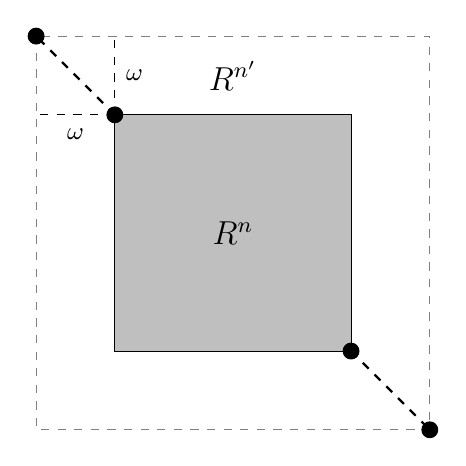
\begin{tikzpicture}[scale=.5]

%set up some coordinates 
%-----------------------
\coordinate (C1) at (0,10); % Outer top left
\coordinate (C2) at (10,0); % Outer bottom right
\coordinate (C3) at (2,8); % Inner top left
\coordinate (C4) at (8,2); % Inner bottom right

%draw figure contents
%--------------------

\draw [fill=lightgray] (C3) rectangle (C4); % Inner rectangle
\draw[dashed, color=gray] (C1) rectangle (C2); % Outer rectangle

\draw [fill] (C1) circle [radius=0.2]; % Outer top left
\draw [fill] (C2) circle [radius=0.2]; % Outer bottom right
\draw [fill] (C3) circle [radius=0.2]; % Inner top left
\draw [fill] (C4) circle [radius=0.2]; % Inner bottom right

\draw[thick,dashed] (C3) -- (C1); % Inner top left to outer top left
\draw[thick,dashed] (C4) -- (C2); % Inner bottom right to outer bottom right

\draw[dashed] (C3) -- (0,8);
\draw[dashed] (C3) -- (2,10);

\draw (5,5) node {\large $R^n$};
\draw (5,9) node {\large $R^{n'}$};

\draw (1,7.5) node {\small $\omega$}; % x1-w
\draw (2.5,9) node {\small $\omega$}; % y1-w

\end{tikzpicture}
\caption{Søgning efter robotten begrænset til $R^n$'s $\omega$ nærmeste pixels.\anders{billedet virker spejlvendt i forhold til en evt. x- og y-akse.}}
\label{tracking:reduction}
\end{figure}

\section{Justering}\label{tracking:adjust}
%Beskrivelse af diverse thresholds og hvilke værdier "der fungerer"
Af de forrige afsnit fås tre variable, der søges justeret således, at de løser de beskrevne problemer tilfredsstillende.
Herunder listes de tre variable, samt en beskrivelse af deres betydning og endelig justering.

Bemærk at værdierne der tildeles variablerne \emph{ikke} er uafhængige.
Ændringer i $\omega$ har således betydning for opdateringshastigheden, hvilken igen har betydning for $\rho$.
Ligeledes har $\rho$ betydning for hvor hvilke pixels der er interessante samt i hvor høj grad der findes støj i de udregnede vægte, hvilket har betydning for $\sigma$ etc.

Værdierne er derfor justeret i takt med, at de forskellige løsninger er implementeret, hvorfor de endelige værdier kan ses herunder.

\begin{description}
\item[Farve afstand (${\boldsymbol{\rho}}$)]
Som nævnt i \cref{tracking:colordiff} er den maksimale afstand mellem to farver 442 (forskellen på sort og hvid).
Den minimale afstand mellem to farver er 0, hvilket er tilfældet for to ens farver.
Altså skal $\rho$ bestemmes mellem disse to.
For den maksimale afstand betragtes alle pixels som interessante, mens det for den minimale kun vil være pixels med den eksakte farve, der søges efter.
Da interessante pixels skal have en farve, der er \emph{tæt på} den søgte, vil $\rho$ have en værdi tættere på 0.
Det er ved forsøg bestemt at:
$$\rho = 50$$
Hvilket angiver, at farver med afstand større end 50 \emph{ikke} er interessante at betragte i løsningen.
%441,672955930063709849498817084

\item[Filter \textit{naboer} ($\boldsymbol{\sigma}$)]
I \cref{tracking:improvements} blev det beskrevet at $\sigma$ højst kan være 8, da en pixel har 8 \emph{naboer}.
Vælges $\sigma = 8$ fremgår det af \cref{tracking:eq:filter} at et sådant filter vil fjerne alt information i billedet.
Vælges derimod $\sigma = 0$ (som er minimum værdi for $\sigma$) vil filteret ingen effekt have.
Det er ved forsøg bestemt at:
$$\sigma = 4$$
Som fjerner alle vægte med færre end 4 interessante nabo-pixels.

\item[Problem reduktion ($\boldsymbol{\omega}$)]
Den kraftigste reduktion af problemets størrelse, uden reduktion af $R^n$, vil være $\omega = 0$ (se \cref{tracking:eq:inflate}) der angiver, at der kun skal søges i den forrige løsnings område, og altså at robotten ikke har flyttet sig.
Dette betyder reelt, at det må gælde at $\omega > 0$.
Der er imidlertid ingen øvre grænse for $\omega$, omend det følger naturligt at jo kraftigere en reduktion der foretages, des hurtigere kan en opdatering ske.
Det er ved forsøg bestemt at:
$$\omega = 5$$
Altså vil firkanten, der indkapslede det forrige resultat udvides med 5 pixels i alle fire retninger (\cref{tracking:reduction}).
Igennem forsøg fremgik det tydeligt at reduktionen i størrelse har en kraftig effekt på opdateringshastigheden.
Derved kunne $\omega$ sættes lavt og en hurtig opdateringshastighed kunne opnås.
I \cref{tracking:updatespeed} beskrives i hvilken grad farvesøgningen forbedredes som følge af $\omega = 5$.
\end{description}

\section{Opdateringshastighed}\label{tracking:updatespeed}
Farvebilleder fra Kinecten kan indsamles på to forskellige måder:
\begin{itemize}
\item I opløsningen 640x480 ved 30 billeder i sekundet
\item I opløsningen 1280x960 ved 15 billeder i sekundet
\end{itemize}

I tabellen herunder præsenteres den opdateringshastighed, der blev opnået i farvesøgning, både med og uden reduktion af problemets størrelse.
Målingerne herunder er kun \emph{omtrentlige}.

{
\newcommand{\mr}[1]{\multirow{2}{*}{#1}}
\newcommand{\ce}[1]{\multicolumn{1}{c|}{#1}}

\begin{center}
\begin{tabular}{| l | r | r |}
\hline
& \ce{Opdateringer} & \ce{Bevægelse}\\
& \ce{pr. sekund} & \ce{pr. opdatering}\\\hline
640x480&\mr{$2-3$}&\mr{$5-10$cm}\\
Ingen reduktion&&\\\hline
640x480&\mr{$29-30$}&\mr{$<1$cm}\\
Med reduktion&&\\\hline
1280x960&\mr{$<1$}&\mr{$20-30$cm}\\
Ingen reduktion&&\\\hline
1280x960&\mr{$12-13$}&\mr{$<1$cm}\\
Med reduktion&&\\\hline
\end{tabular}
\end{center}}
%
%%Bemærk at implementationen af farve-afstand og afgrænset område forudsætter 'høj' fps
%
%Distance threshold: \rho
%Neighbour threshold: \sigma
%Inflation 'threshold': \omega
%
%640x480 - NoBounds
%3-4fps, 5-10cm
%
%1280x960 - NoBounds
%<1fps, 20-30cm
%
%640x480 - Bounded
%29-30fps, <1cm
%
%1280x960 - Bounded
%12fps, <1cm
%